\documentclass[programming,a4paper,12pt,twosided]{myassignment}
\usepackage{cleveref}
\hypersetup{hidelinks}

\title{CPS 2003 - Systems Programming}
\subtitle{Assignment}
\author{Mark Said Camilleri}
\id{306697M}
\course{B.Sc Computing Science}
\university{University of Malta}
\logo{University_of_Malta_Logo.eps}
\lecturer{Dr Alessio Magro}
\date{26th May 2017}
%\addbibresource{bibliography.bib}

\begin{document}
\maketitle
\abstract{The aim of this assignment was to make a multiplayer snake game with C. This report serves to compliment the source code submitted as well as explain further the thought and design process behind it and evaluate the code submitted}
\tableofcontents
\chapter{Design}
The system was designed so that it consists of two programs, the sever, whcih will take care of the game logic for all the clients connected to it, and the client, which will take care of passing user input to the server and displaying the map and scores to the user.
\section{Communcation}
These two programmes were designed to interact together using sockets over the TCP protocol. This was done via the system calls defined in \verb|sys/socket.h|. Figure \ref{fig:interaction} shows the sequence of how communication through the socket is established.

This implementation meant that the server has to communicate different types of data to the clients. As a result, an application-level protocol was established such that the server sends the size of the data, the type of the data (in the form of an integer) and then the data itself. The first 2 have a fixed sze, whereas the size sent is then used as a buffer size for the data, eliminating any buffers that are too big or too small.

The type of data has to be communicated as well since the client would need to decide what to do with it once the data is received. If it is a special server message, such as ``Server Down'', ``Player Lost'' or ``Player Won'', then the client treats those in a different way. Similarly, the client would need to treat the map different to the snake it recieves.

The server was designed to make use of a 2D integer array to represent the map and differenciate between empty tiles, tiles with a snake on them and tiles with fruit on them. The server also held a dynamic array (created as a struct) to store all the snakes in play. Furthermore, a linked list was built for the list storing all the client's connections such that functions could then be defined recursively over this structure. 

\begin{figure}
  \centering
  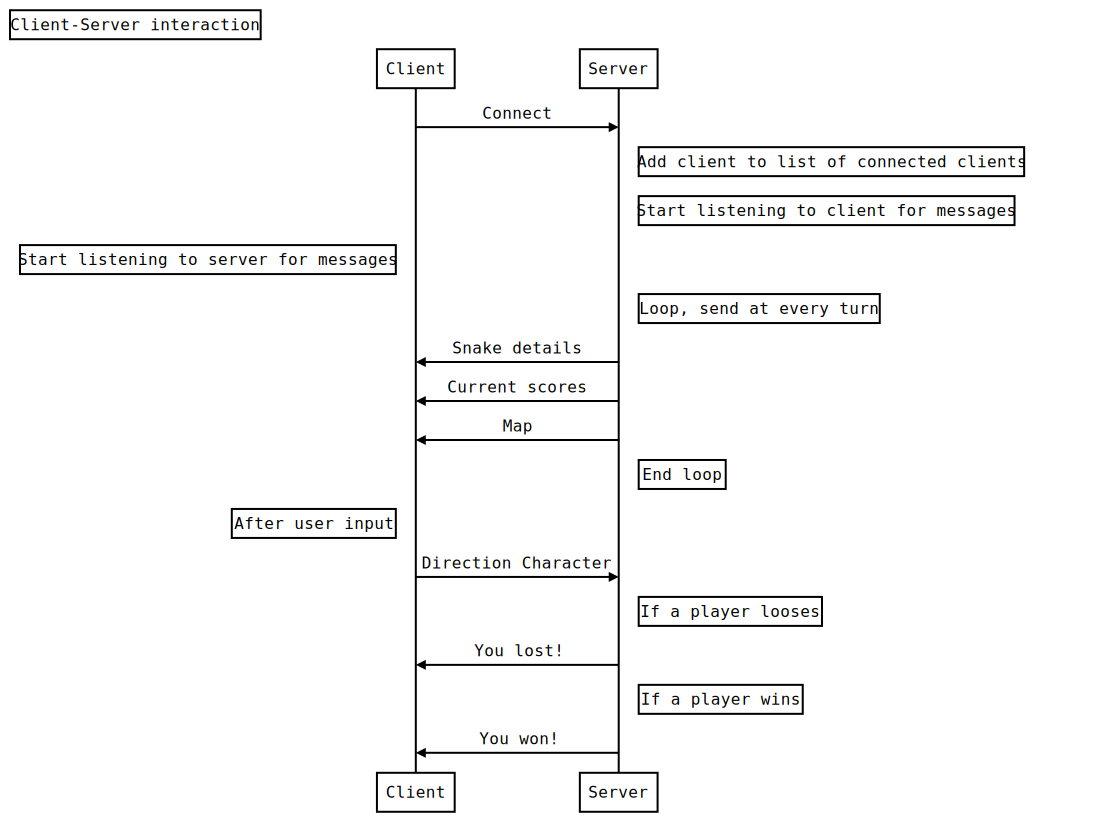
\includegraphics[width=\textwidth]{interaction}
  \caption{The client and server interactions}
  \label{fig:interaction}
\end{figure} 

\section{User Interface}
\emph{ncurses} was used to displaly the game to the user at the client side. It was designed and implemented to look like the mockup in Figure \ref{fig:mockup}, where the main area of the screen would be focused on part of the game map, a small section of the screen would be dedicated to guiding the player and another small section of the screen would display the scores of the top players that would fit. 

This was done using \emph{ncurses}' windows implementation, which splitting the screen provided (terminal) into smaller independant windows. This made sure that no window overlapped each other.

\begin{figure}
  \centering
  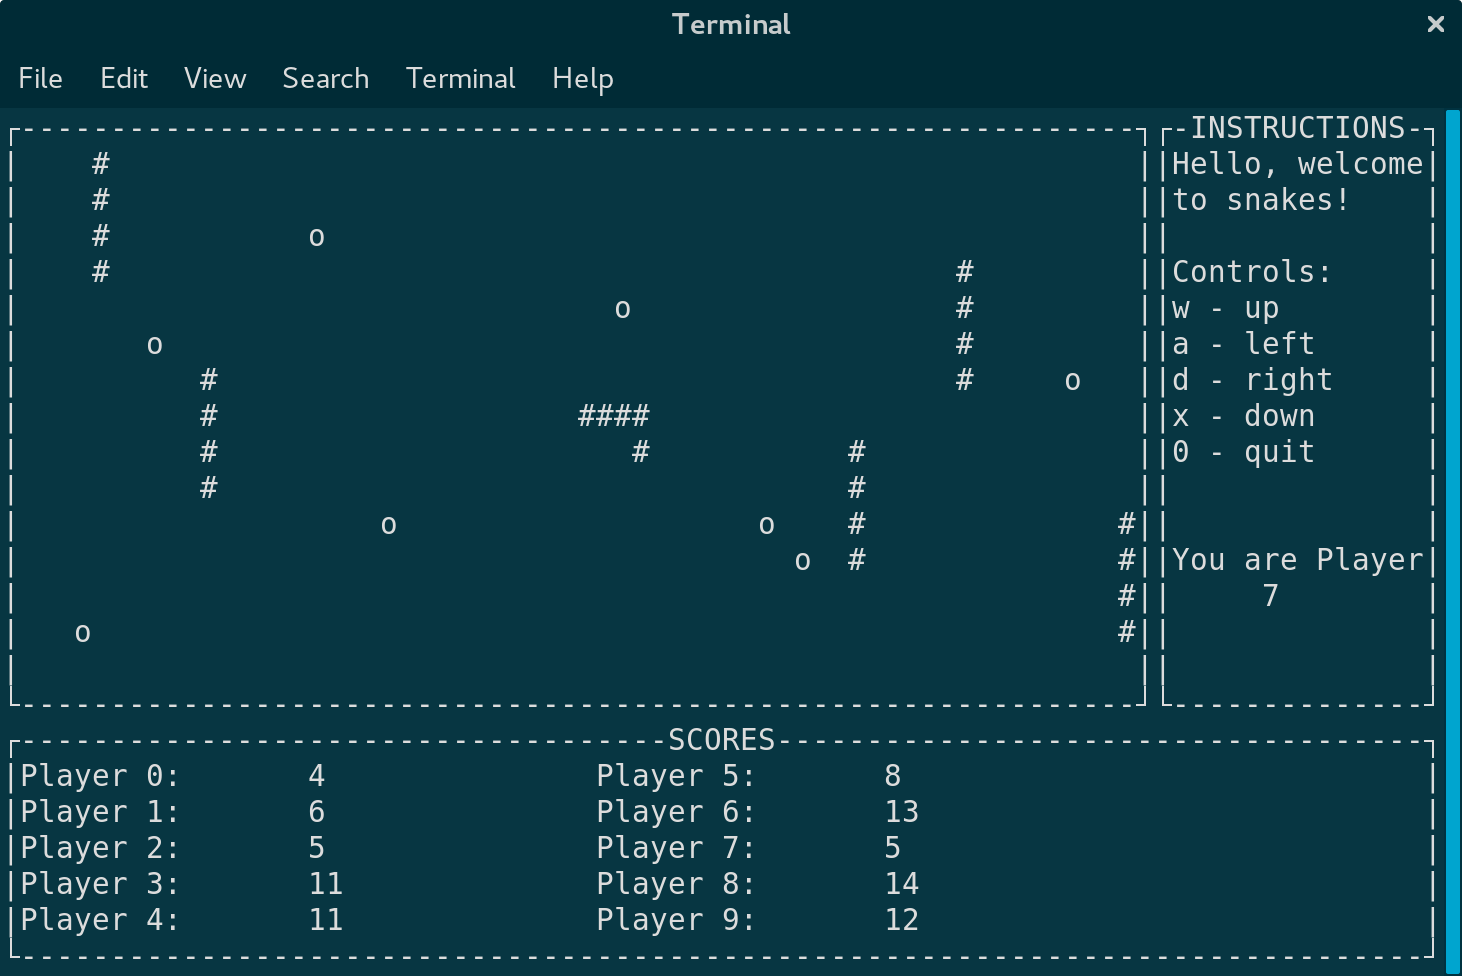
\includegraphics[width=\textwidth]{terminal}
  \caption{The mockup user interface}
  \label{fig:mockup}
\end{figure} 

\chapter{Implemetation}
The system is implemented to be multi-threaded. The server starts, initializes a socket to be used by the clients to connect to it to play the game. It will then proceed to intialize and run the game. A seperate thread is created to let the server accept connections while the game is running. For each connection accepted, a snake is create another thread is also created to read and react to that client's input.

The main thread, will initialize the game board and start the game. On each turn, each snake is moved one character to the direction it's facing. Should a snake hit the edge, another snake, or itself, that player loses and exits the game. Should a snake go on a fruit tile it grows by one character. The game ends when a snake would have reached fifteen characters. To ensure safe use of resources between threads, mutexes have been used.

\chapter{Evaluation}
Unfortunately, due to time constraints, while I have done my best to make this system free of race conditions, free of bugs and fault tolerant, it is evident that bugs are very much presnet in the system. These were found by testing the system first hand, and using valgrind to detect some issues as well.

Unfortunately, the game map is not being displayed properly to the user (I guess this would be a blind version of snakes then). Furthermore, when a game is in progress,  the system does not seem to allow more clients to join, despite this being allowed in theory. This could be due to where and when the mutexes are locked and unlocked, whcih would lead in not enough time for the thread accepting connections to lock the mutex. It would be beneficial to check the order of mutex locks and unlocks as well as which ones are being used.

Lastly, it has also been noticed that at the end of the game, the server attempts to send data to disconnected clients, sometimes resulting in a segmentation fault whcih could mean a memory leak.
\end{document}
